
%%%%%%%%%%%%%%%%%%%%%%%%%%%%%%%%%%%%%%%%%%%%%%%%%%%%%%%%%%%%%%%%%%%%%%%%%%%%%%%%
%%%%%%%%%%%%%%%%%%%%%%%%%%%%%%%%%%%%%%%%%%%%%%%%%%%%%%%%%%%%%%%%%%%%%%%%%%%%%%%%
\section{Percepção da informação}
\index{Aprendizagem!Percepção}
\label{sec:percepcionaprendizagem}

\begin{wrapfigure}{r}{0.5\textwidth}
  \centering
    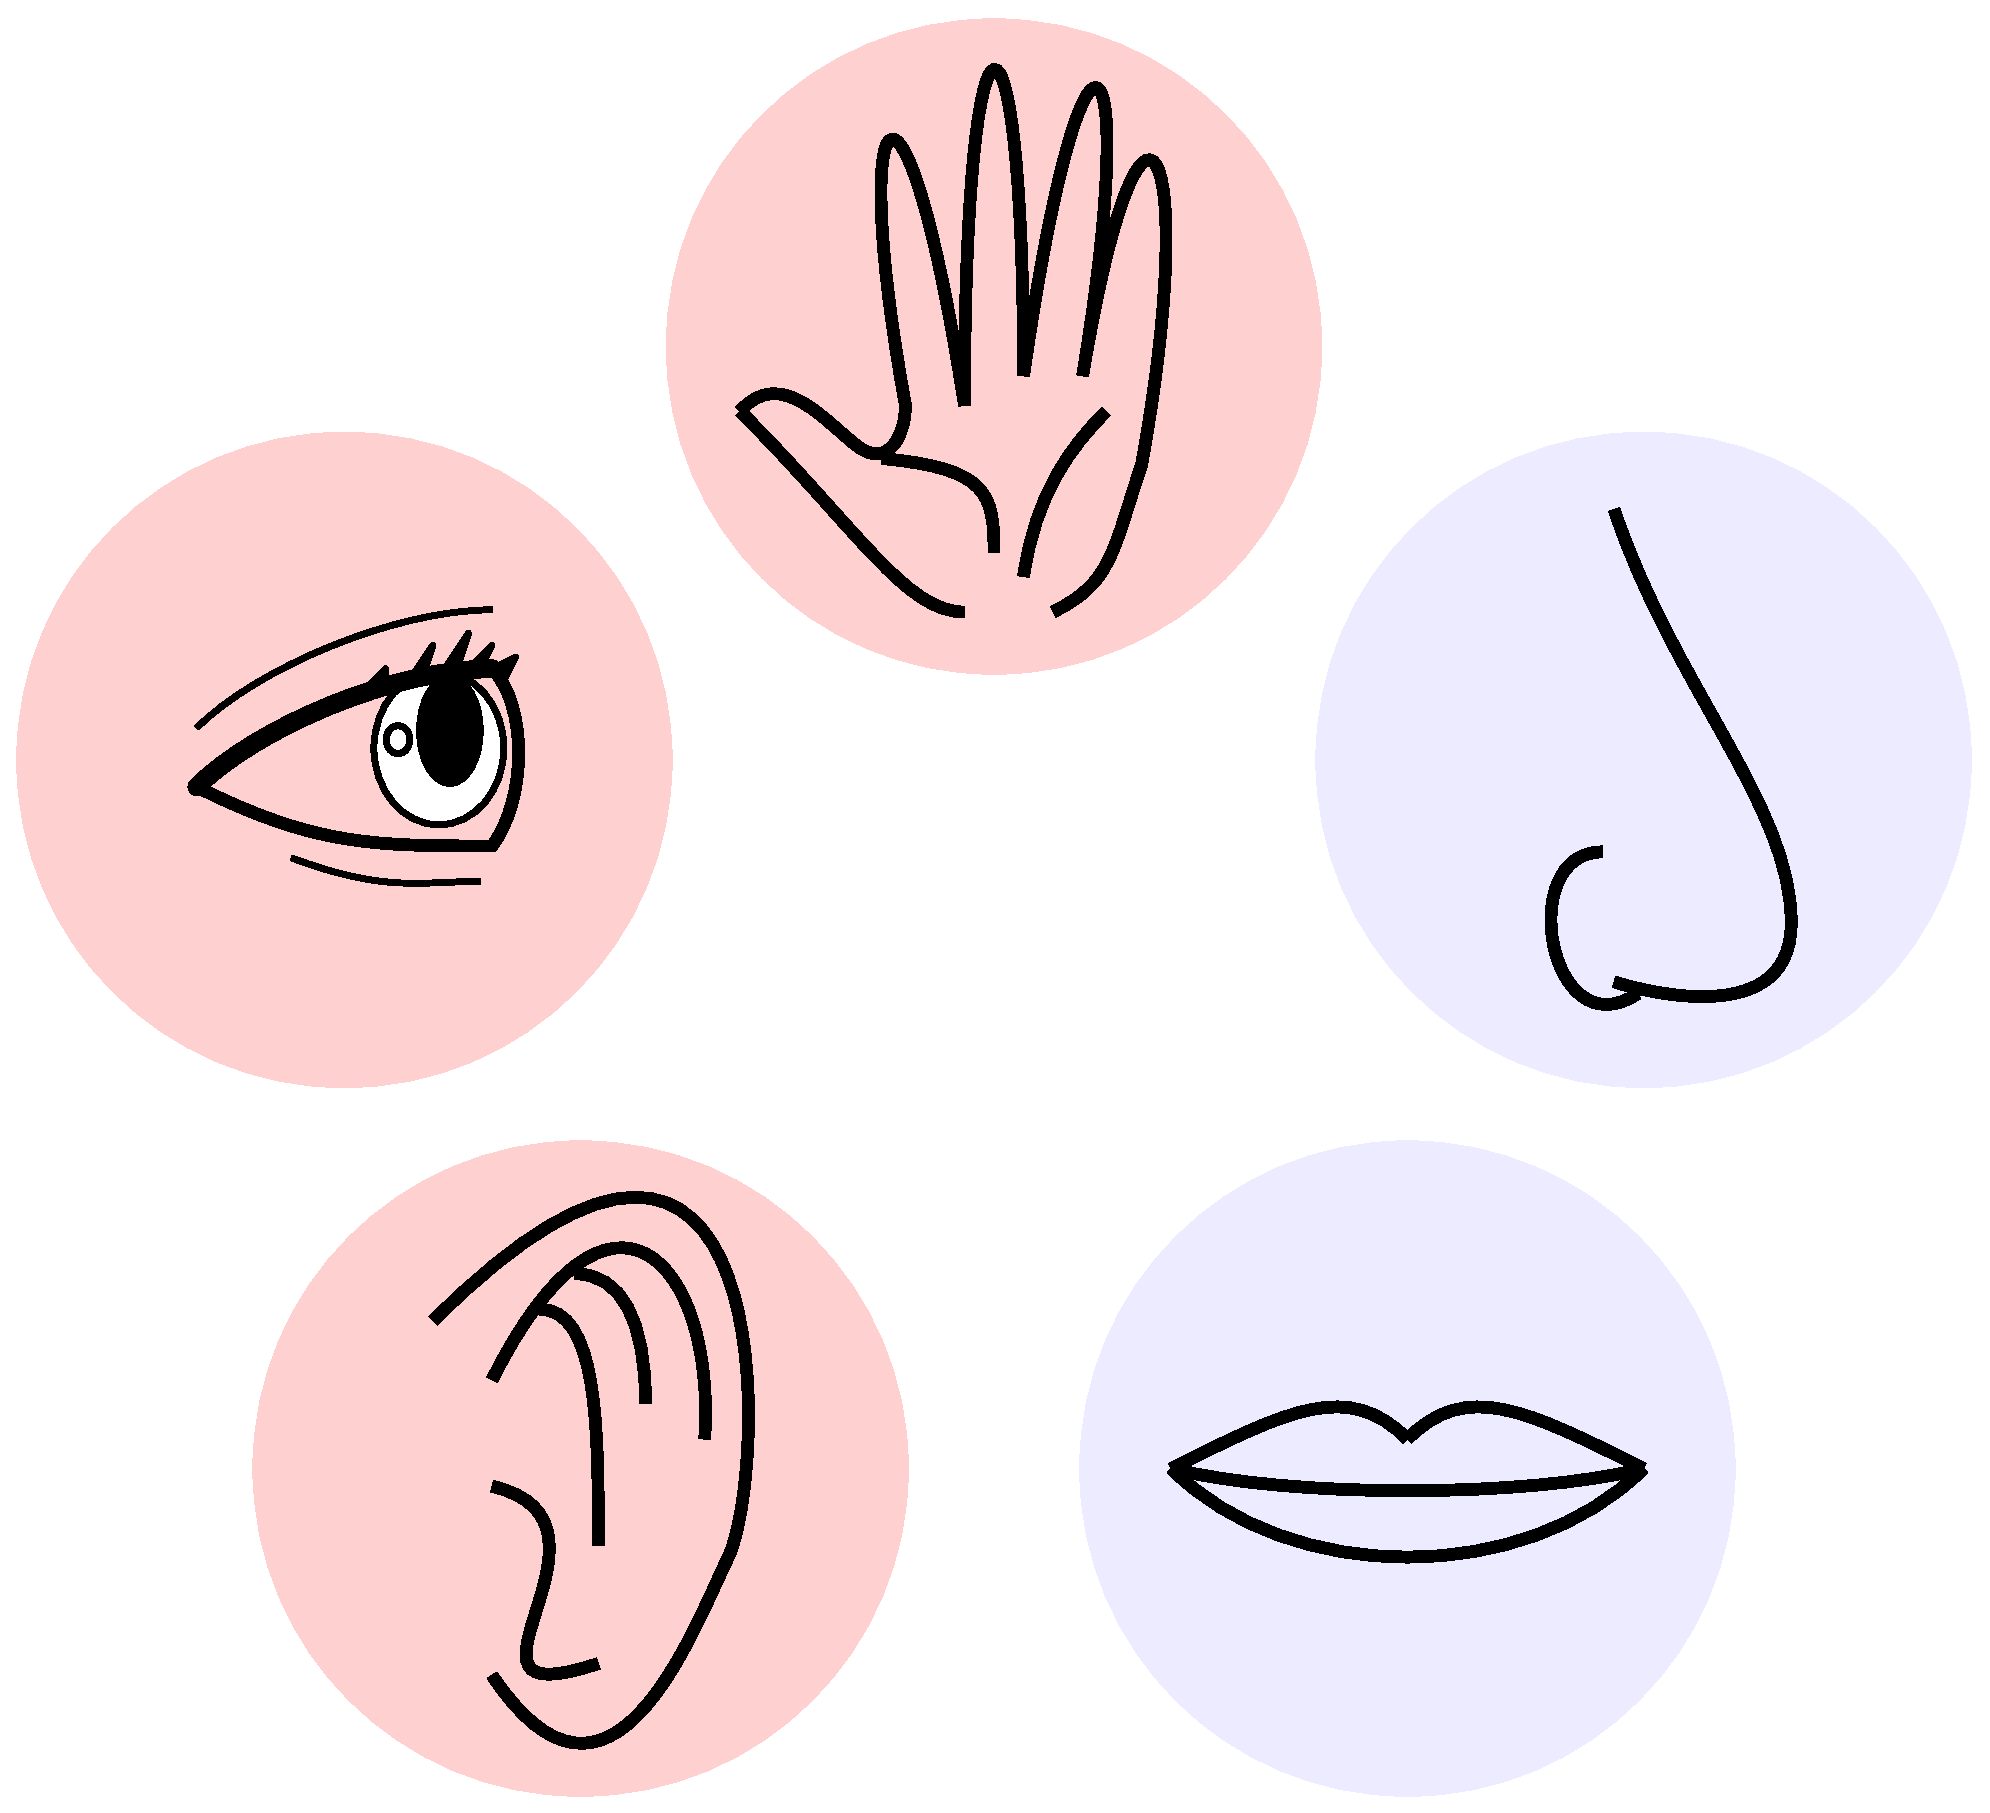
\includegraphics[width=0.48\textwidth]{chapters/cap-learning/sentidos.eps} 
  \caption{Sentidos do corpo.}
\label{fig:5sentidos}
\end{wrapfigure}
O ser humano entende o mundo que lhe rodeia mediante o uso do seus sentidos,
ver Figura \ref{fig:5sentidos},
de modo que suas percepções podem ser de caráter \cite[pp. 28]{ready2010pnl}:
\begin{itemize}
\item visual (olhos), 
\item auditivo (ouvidos),
\item cinestésico (emoções e tato), 
\item olfativo (nariz) e
\item gustativo (gusto).
\end{itemize}

Entre todas estas possíveis fontes de informação,
pelo geral, quando estamos em nosso momento de maior estresse,
cada um de nós manifestamos preferencia por alguma destas 5 fontes de informação;
este sentido preferenciado é conhecido como ``sistema figurativo'' ou ``sistema de representação primordial''
\cite[pp. 28]{ready2010pnl}.


Seja metafórica ou real uma fonte de conflito, o estresse sempre estará presente 
e nosso corpo acudirá preferencialmente a nosso sistema de representação primordial para obter informação.
Quando tentamos alcançar a competência numa área desfavorável para nós\footnote{Estágio 
2 de nosso aprendizado visto na Pag. \pageref{ref:IncompetenciaConsciente}.},
podemos atingir o estresse, consequentemente nosso corpo acudirá com atenção a 
nosso sistema de representação primordial;
pelo que é interessante fazer um exame de autoconhecimento, 
para poder saber qual é este sentido em nós e assim otimizar nosso processo de aprendizagem.

É interessante ressaltar da Figura \ref{fig:5sentidos}, 
que se tomamos o papel de professor  numa sala de aula de dança, 
geralmente exploramos 3 destes sentidos
(visual, auditivo, e cinestésico), 
deixando fora a percepção olfativa e gustativa, 
pelas obvias dificuldades pedagógicas que estes enfoques carregariam num modelo de sala de aula tradicional;
porém são possibilidades de enfoques pedagógicos válidas.
Por outro lado, pensando nos três sentidos que são mais aproveitáveis na sala de aula,
devemos ter cuidado de que a informação que entreguemos aos estudantes, 
estejam adequadamente proporcionadas na forma visual, auditiva, e cinestésica.
\begin{tcbattention}
Devemos evitar cometer o erro de só focar nossa aula de dança em explicar e mostrar um movimento (visual, auditivo),
descuidando o treinamento das repetições (cinestésico), 
provocando dessa maneira que as pessoas que tenham um sistema de representação primordial cinestésico, 
saiam pouco favorecidas na quantidade de informação percebida na nossa aula.
\end{tcbattention}


\begin{figure}[!ht]
\begin{elaboracion}{Ditado chines}
Existe um velho ditado chines atribuído a Confúcio \cite[pp. 60, 63]{AprendendoInteligencia2008} \cite[pp. 9]{abe2002introducao}:

\begin{center}
    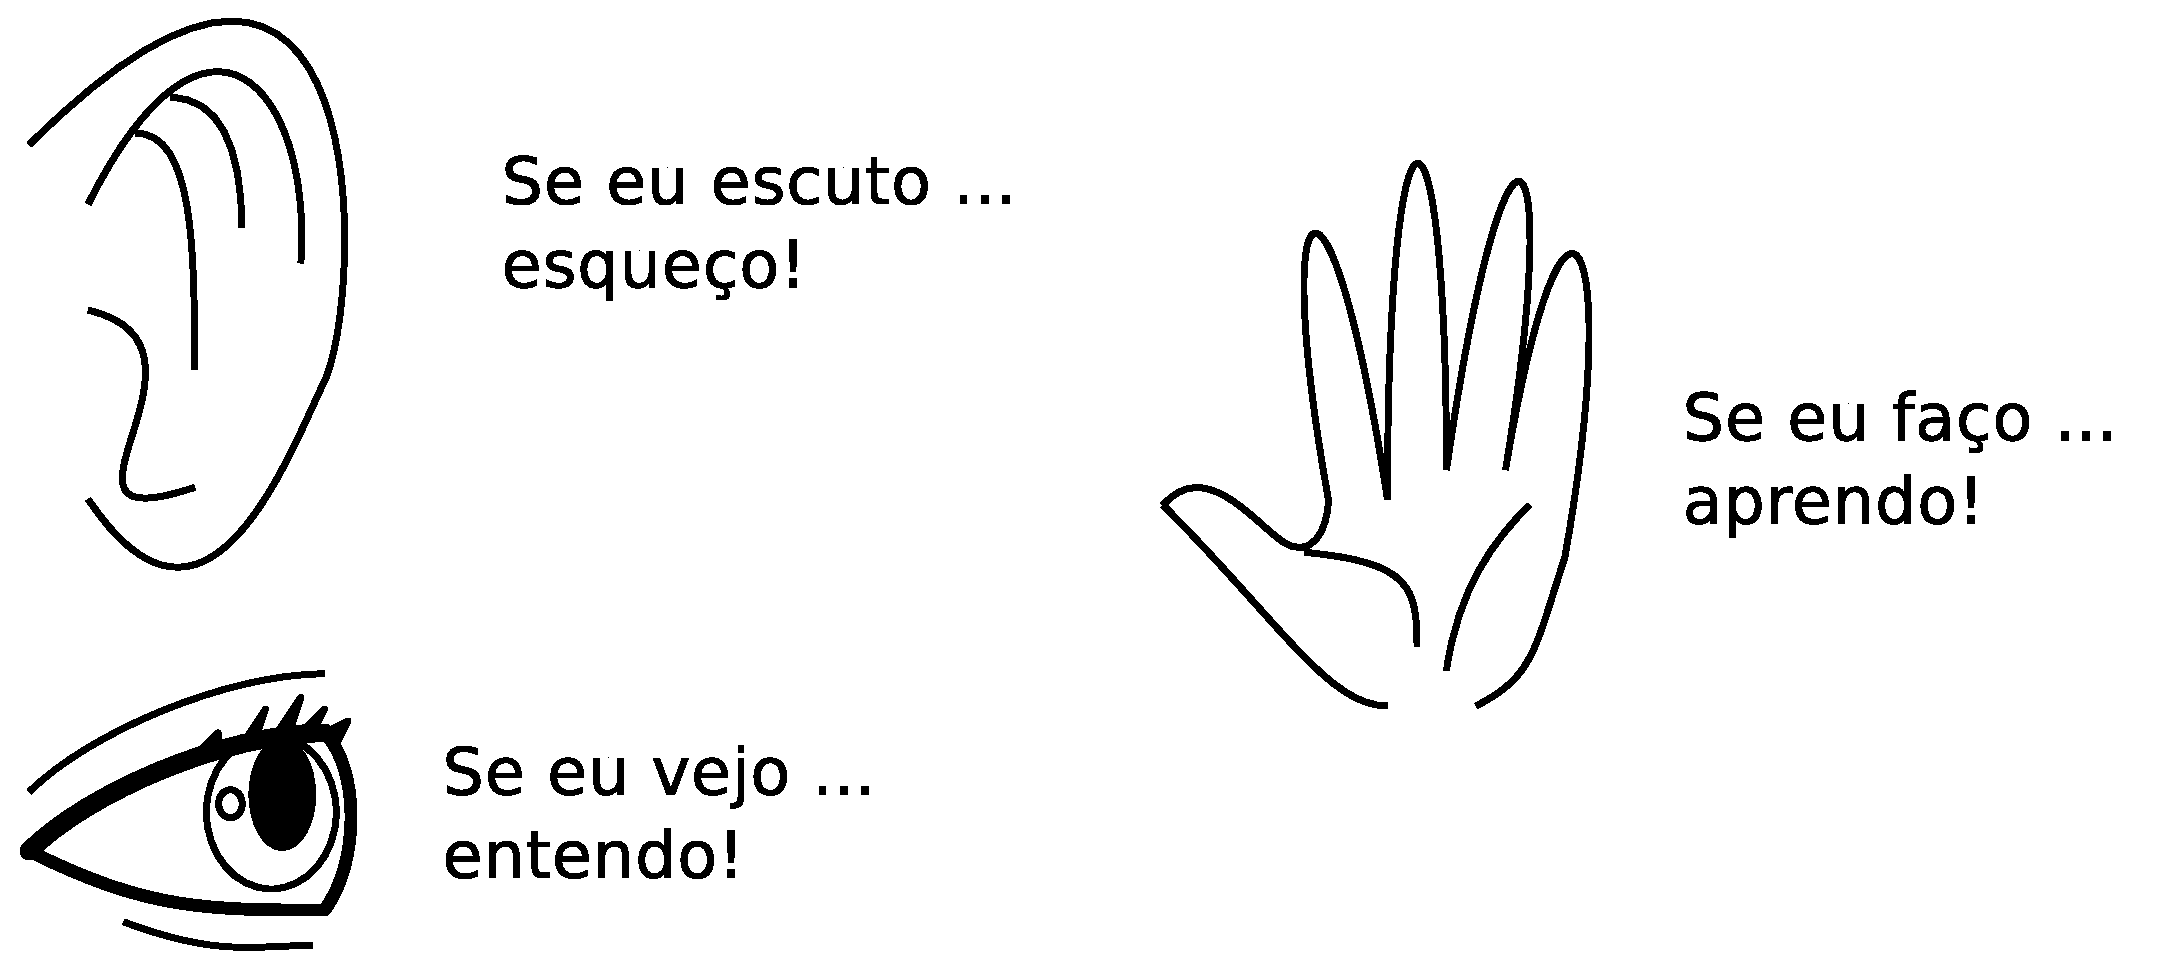
\includegraphics[width=0.7\textwidth]{chapters/cap-learning/ditadochines.eps}
\end{center}
\end{elaboracion}
\end{figure}

É importante lembrar que as caraterísticas visual, auditivo, cinestésico, olfativo e gustativo,
nos indicam como percebemos a informação, mas não como esta é armazenada, retida e evocada no nosso cérebro,
pois estas caraterísticas correspondem ao estudo da memória.  
Porém, existe um ``modelo de multiarmazenamento de memória''\footnote{A 
proposta de Atkinson e Shiffrin é um modelo mental para representar o fluxo da informação, 
e não deve ser entendido como uma proposta de esquema com estruturas fisiológicas separadas.}, 
proposto por Richard Atkinson e Richard Shiffrin (1968),
também chamado ``modelo de memória modal'' (comum ou normal),
que explica a relação que existe entre a informação recebida pelos 5 sentidos 
e os seguintes três sistemas de armazenamento  
\cite{10.2307/24922803} \cite[pp. 158]{sternbergpsicologia} \cite[pp. 32]{de2000comprension} \cite{pake2019psicologia}:
\begin{itemize} 
\item \textbf{Memória sensorial (Registro sensorial)}: A informação dos registros sensoriais duram na memoria um curto período de tempo, menos que 2 segundos.
e tem um espaço de almacenamento limitado.
\item \textbf{Memória de curto prazo}: Para mais detalhes ir a Seção \ref{sec:memoria:curto}.
\item \textbf{Memória de longo prazo}: Para mais detalhes ir a Seção \ref{sec:memoria:longo}.
\end{itemize}

\begin{figure}[!h]
  \centering
    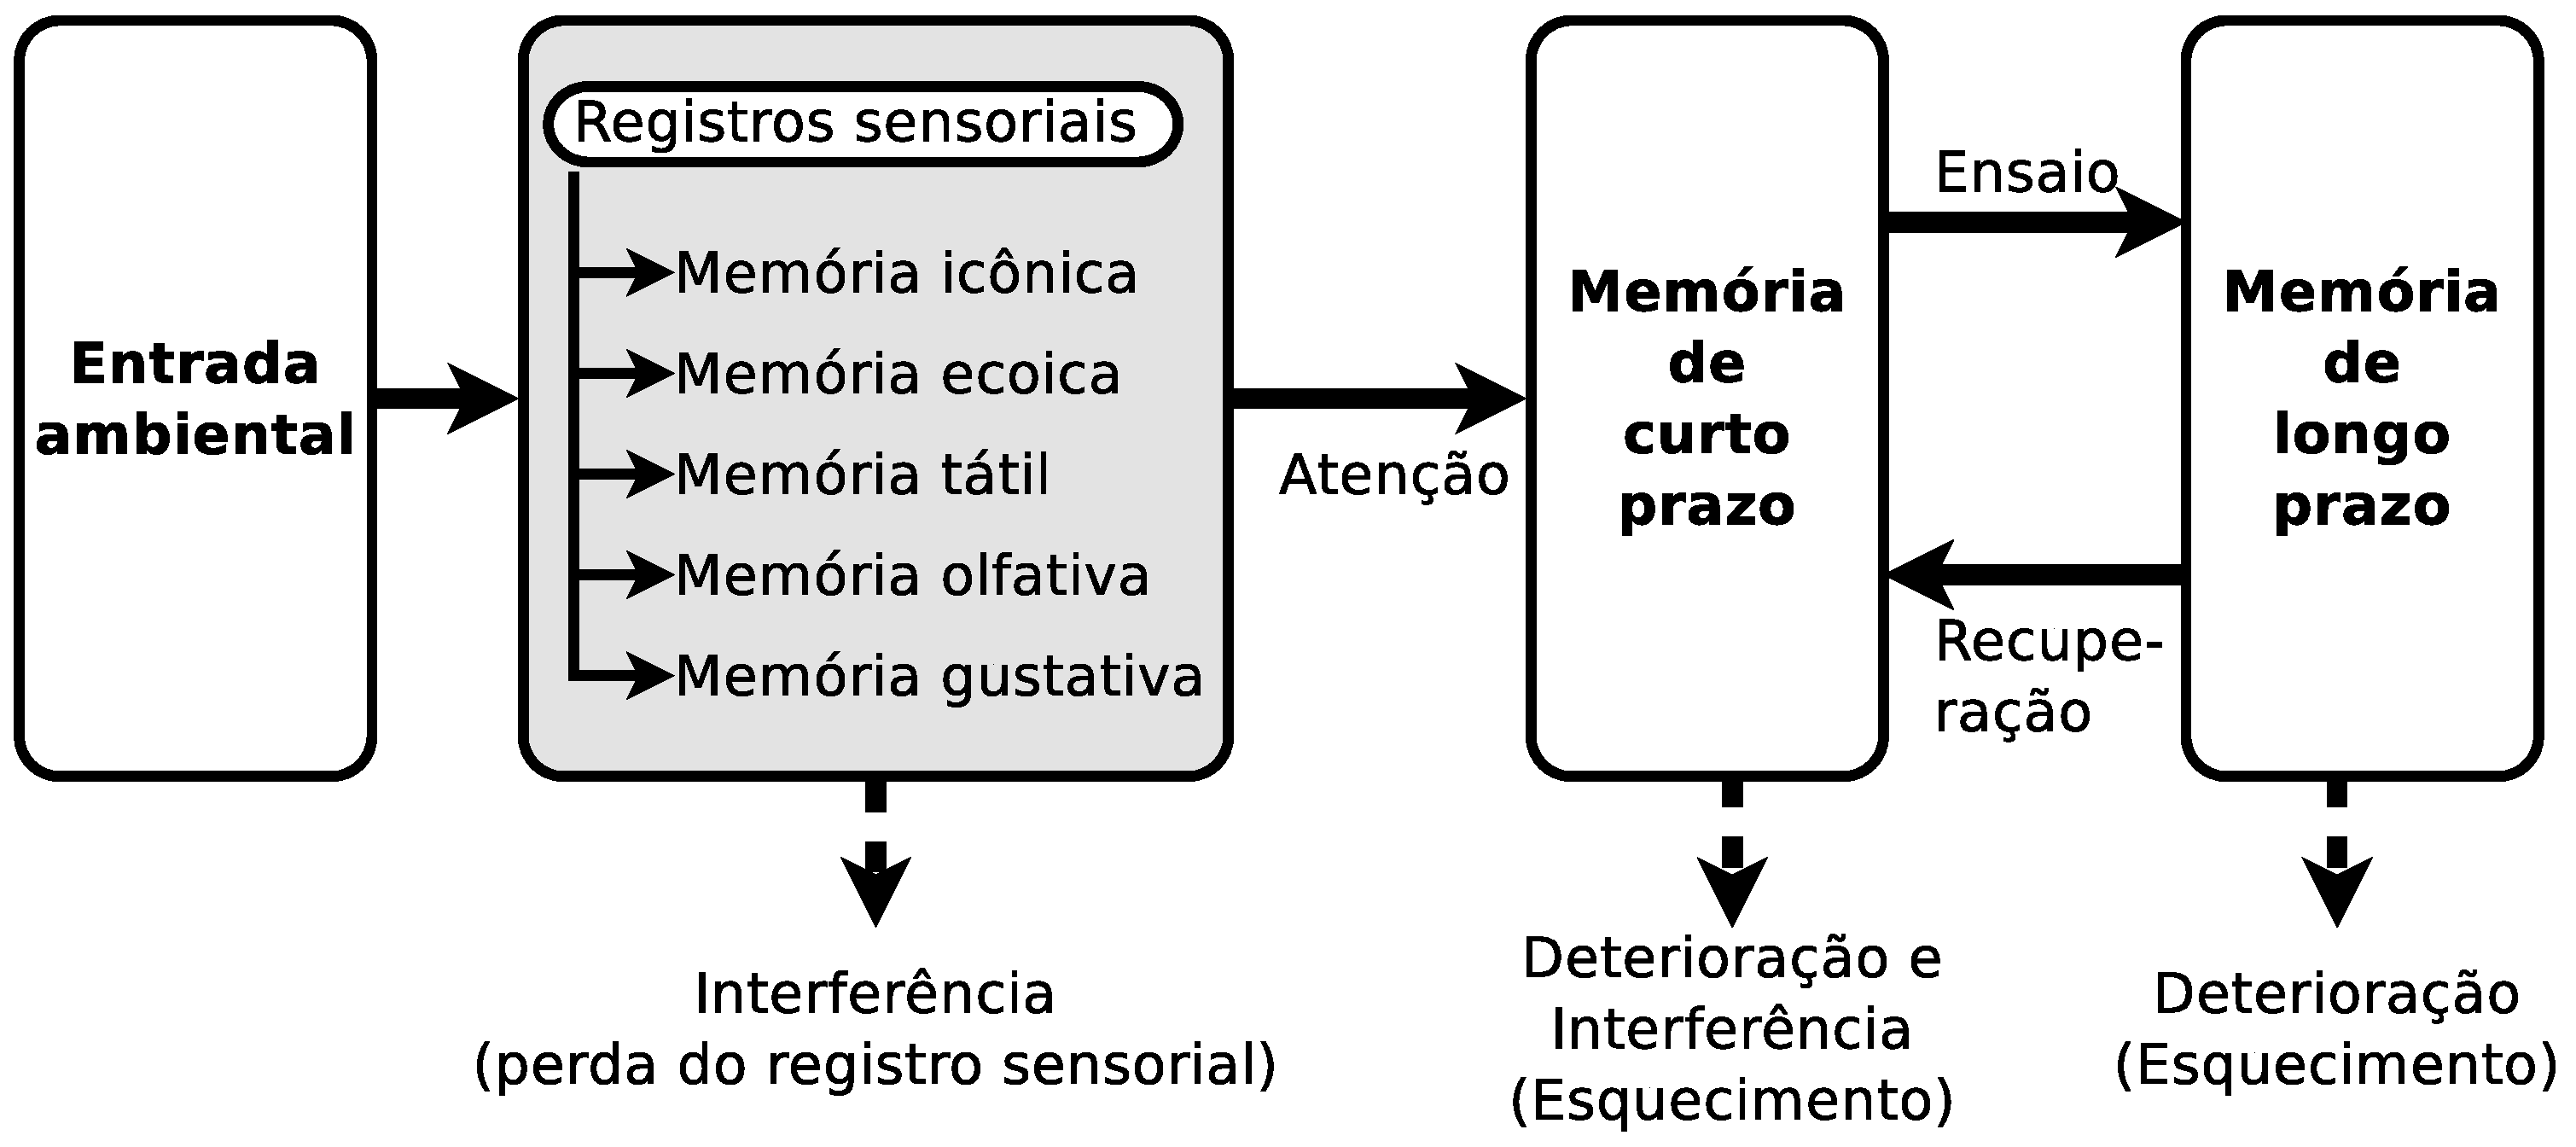
\includegraphics[width=\textwidth]{chapters/cap-learning/sentidos-memoria.eps} 
  \caption{Modelo de multiarmazenamento de memória.}
\label{fig:sentidos-memoria}
\end{figure}
\index{Aprendizagem!Modelo}
O modelo de multiarmazenamento de memória pode ser visto no diagrama da Figura \ref{fig:sentidos-memoria},
onde a ``entrada ambiental'' corresponde aos 5 sentidos;
este bloco entrega a informação percebida pelos sentidos aos ``registros sensoriais'', 
que realizam uma cópia instantânea,
de modo que existe um registro para cada sentido \cite[pp. 158-159]{sternbergpsicologia}  \cite{pake2019psicologia}.
\begin{itemize}
\item Memória icônica: Para a visão.
\item Memória ecoica: Para a audição.
\item Memória tátil: Para o tato.
\item Memória olfativa: Para o olfato.
\item Memória gustativa: Para o paladar.
\end{itemize} 

Filtramos a informação indesejada quando prestamos atenção a estes registros sensoriais,
e levamos estas informações à memoria de curto prazo  e 
à de longo prazo
\cite[pp. 158-159]{sternbergpsicologia} \cite{pake2019psicologia}.
\begin{tcbattention}
É importante ressaltar que o modelo proposto por Richard Atkinson e Richard Shiffrin, 
com três receptáculos, 
não é a única maneira para representar o funcionamento da memória \cite[pp. 159]{sternbergpsicologia}.
\end{tcbattention}
